%!TEX root = ../main.tex
\chapter{Návrh riešenia}
Táto kapitola sa bude venovať popisu funkcionality projektu z pohľadu používateľa v týchto bodoch:

\begin{itemize}
  \item Štruktúra aplikácie na strane klienta a servera
  \item Vysvetlenie princípov fungovania herného sveta
  \item Minimálne požiadavky pre spustenie aplikácie
  \item Priblíženie si navrhovaných riešení niektorých problémov
\end{itemize}



\section{Štruktúra aplikácie}
\subsection{Klient}
\subsubsection{Prihlasovacia obrazovka}
Androidová aplikácia po spustení používateľovi ponúkne prihlasovaciu obrazovku obr.~\ref{fig:klient_login}, vďaka ktorej sa môže používateľ prihlásiť, ak zadá potrebné prihlasovacie údaje a adresu herného serveru, na ktorý sa plánuje pripojiť. Pokiaľ používateľ nemá vytvorený herný účet na danom serveri, môže sa jednoducho zaregistrovať pomocou registračného tlačidla. Po úspešnom prihlásení sa stiahnu nastavenia hry ako je napríklad názov hry. 
\begin{figure}[h]
  \centering
  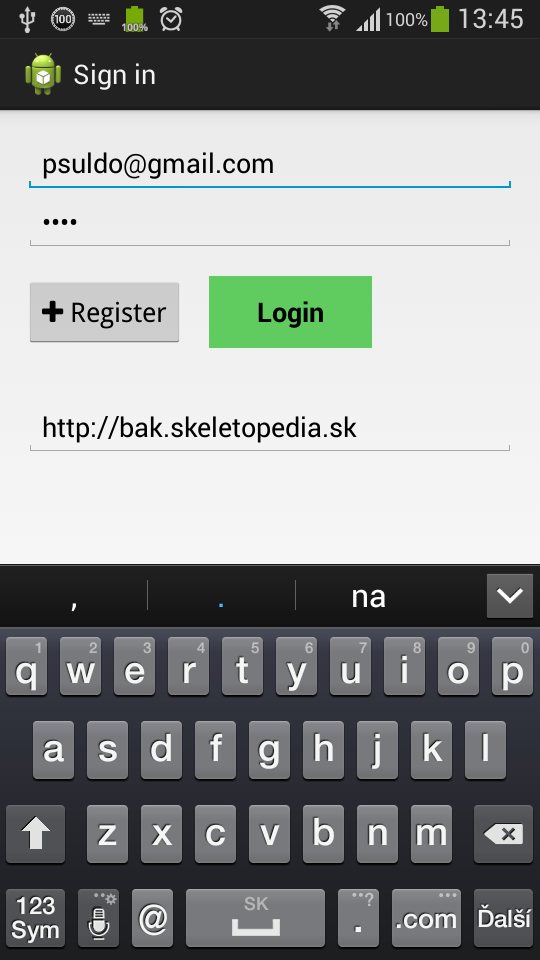
\includegraphics[height=10cm]{mainmatter/imgs/klient_login.png}
  \caption{Prihlasovacia obrazovka pre hru}
  \label{fig:klient_login}
\end{figure}
\subsubsection{Hlavná obrazovka}
Obrazovka, ktorá sa objaví používateľovi po úspešnom prihlásení slúži ako odrazový mostík pre interakciu s herným svetom. Ak nie je nastavené inak, automaticky zistí názvy herných obrázkov zo serveru a začne ich sťahovat do aplikácie podľa toho, ktoré chýbajú. O postupe informuje používateľa dialógovým oknom. Na hlavnej obrazovke sa nachádza tlačidlo na manuálne zistenie informácii o hernom svete, ak by používateľ chcel získať aktuálnejšie informácie. Ďaľej tu nájdeme tlačidlo na oskenovanie QR kódu do aplikácie, pre zistenie či naskenovaný QR kód reprezentuje úlohu alebo odmenu. Tlačidlo nastavenia spustí obrazovku s nastaveniami mobilnej aplikácie. Tlačidlo prijať objekt, slúži na spustenie obrazovky, ktorá sa stará o nadviazanie Bluetooth spojenia a prijatie objektu od darcu. Posledné tlačidlo, ktoré sa nachádza na tejto obrazovke je tlačidlo slúžiace na odhlásenie prihlaseného hráča a následného otvorenia prihlasovacej obrazoky. Text tlačidiel je vizuálne doprevádzaný obrázkami pre intuitívnejšie pochopenie ich funkcionality. Horná horizontálne posúvna lišta ponúka menu pre hráča

\subsubsection{Nastavenia}
Táto časť aplikácie slúži na nastavenie správania herného klienta. Používateľ si tu môže nastaviť hernú prezývku. Tiež sa môže rozhodnúť ako často aktualizovať dáta pre aktuálnu polohu, poprípade vypnúť túto aktualizáciu a ponechať len manuálnu. Ďaľším nastavením je možnosť automatickej aktualizácie herných obrázkov pri spustení, ktoré konkrétna hra využíva. Nachádza sa tu aj tlačidlo pre prípad, že používatel chce vynútiť aktualizáciu týchto obrázkov.

\begin{figure}[h]
  \centering
  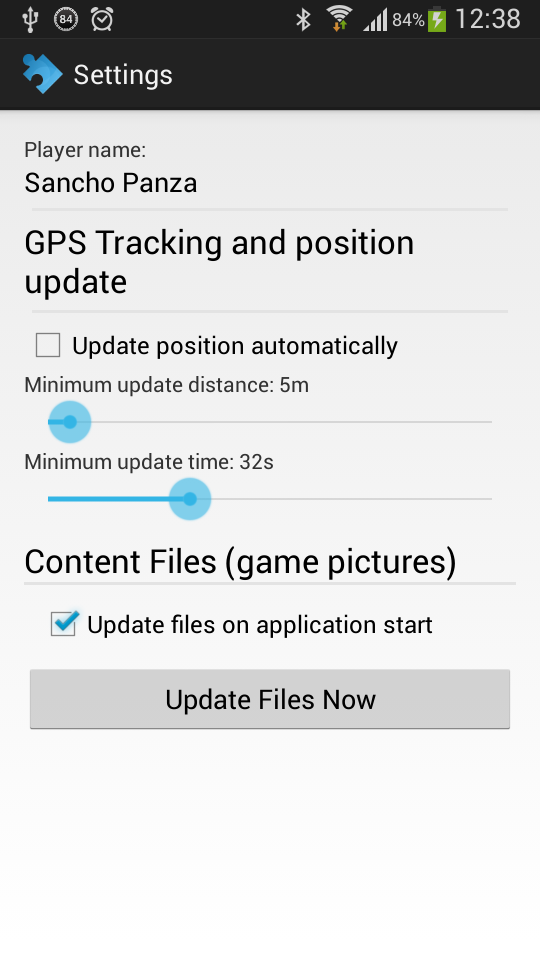
\includegraphics[height=10cm]{mainmatter/imgs/klient_settings.png}
  \caption{Používateľ môže nastaviť správanie aplikácie}
  \label{fig:klient_settings}
\end{figure}



\subsubsection{Úlohy}
K tomu aby mal hráč prehľad o úlohách bola vytvorená obrazovka s úlohami. Možno si na nej teda pozrieť aktuálne úlohy, ktoré hráč môže prijať. Ako ďaľšie sú zobrazené prijaté teda aktívne úlohy, ktoré už boli prijaté hráčom a teraz prebieha ich riešenie. Poslednou kategóriou sú kompletné, ciže úspešne dokončené úlohy, v ktorých sa podarilo hráčovi úspešne splniť zadania daných úloh. Tieto tri kategórie sí filtrovatelné pomocou troch tlačidiel. Každé jedno tlačidlo má dva stavy a je pridelené ku svojej kategorii. Ak je tlačidlo zapnuté zobrazí úlohy takého stavu, ktorému prislúcha a vice versa.

\subsubsection{Detail úlohy}
Obrazovka s detailom úlohy ponúka informácie pre hráča pre jej splnenie. Nájdeme tu názov úlohy, jej popis so zadaním, obrázok jej prislúchajúci a tlačidlá. Tlačidlá sa zobrazujú podla stavu úlohy. 

Ak je úloha dostupná je viditeľné tlačidlo pre jej prijatie. 
Aktívna úloha, zobrazuje tlačidlo na odobratie úlohy a jej splnenie. Hotová úloha zakáže používanie tlačídla pre splnenie úlohy. Podľa typu úlohy sa zobrazujú komponenty na obrazovke. Pri úlohe, ktorá vyžaduje textovú odpoveď je viditeľný textový vstup, do ktorého hráč može písať. Ak má úloha nastavený časový limit, zobrazuje sa sekundový odpočet, ktorý je znázornený pomocou komponentu postupu ~\ref{fig:klient_deatilUlohy}.
\begin{figure}[h]
  \centering
  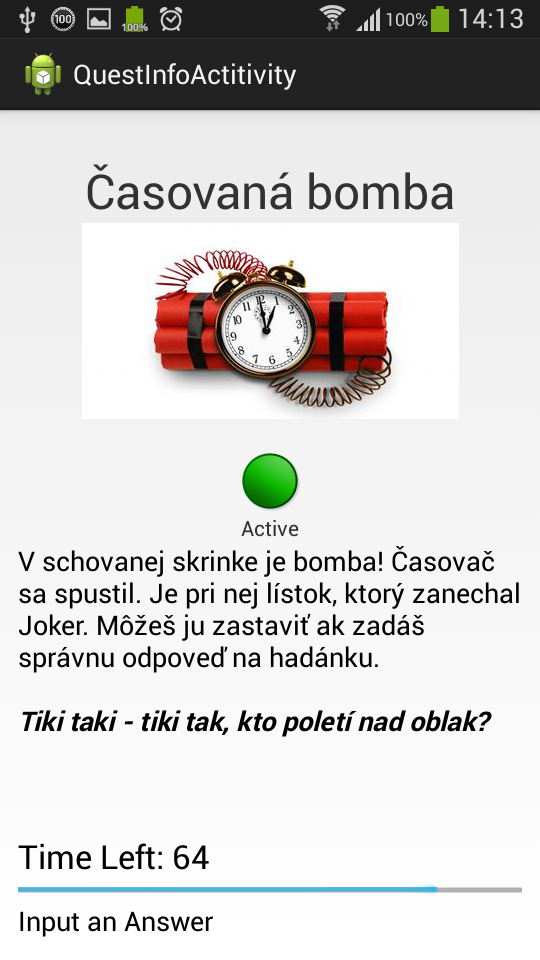
\includegraphics[height=10cm]{mainmatter/imgs/klient_questrunning.png}
  \caption{Detail úlohy na čas vyžadujúcej textovú odpoveď}
  \label{fig:klient_deatilUlohy}
\end{figure}

\subsubsection{Atribúty}
Každý hráč si môže pozrieť zoznam svojich aktuálnych atribútov, ktoré nadobudol. Atribúty sú zobrazené pod sebou. Každý atribút má svoj obrázok, názov a číselnú hodnotu, ktorou informuje hráča ako postupuje v hre.

\subsubsection{Inventár}
Hráči so sebou nosia v inventári objekty. Objekty sú na tejto obrazovke inventára zobrazené ako býva zvykom v počítačových hrách - v mriežke uložené vedľa seba, kde pri jednotlivých položkách tohto zoznamu je zobrazené ako objekty vyzerajú a pod obrazkami sú názvy a počty jednotlivých objektov. Kliknutím na konkrétny objekt sa otvorí obrazovka s detailnejším popisom objektu.

\subsubsection{Detail objektu}
Detail objektu  ak má hráč záujem zistiť viac informácii o objekte, napríklad prečítať si detailný popisok, či pozrieť si obrázok na . Ak má hráč záujem odoslať práve vybraný objekt, niektorému druhému hráčovi v blízkosti, môže tak urobit pomocou tlačidla na darovanie objektu. To otvorí obrazovku na pripojenie zariadení pomocou technológie Bluetooth.

\subsubsection{Zoznam aktuálnych regiónov a detail regiónu}
Aby hráč mal lepšiu predstavu, kde sa v hernom prostredí pohybuje je mu ponúknutý zoznam regiónov, v ktorých sa práve nachádza. Jednotlivé regióny sú zobrazené velkým obrázkom a názvom regiónu. Pri prekliknutí na konkrétny región sa zobrazí obrazovka s detailenjším popisom regiónu, tak ako je to aj pri objektoch.

\subsubsection{Mapa}
Mapa slúži ako oporný bod  pre lepšiu orientáciu pri hraní hier v teréne. Tiež informuje hráčov o tom, v ktorých regiónoch sa hráč nachádza. Ak sa hráč nachádza v regióne, tak sa na mape zobrazí značka s názvom regiónu a farebne vyznačená plocha, ktorá určuje hranice regiónu.

\subsubsection{Obrazovka posielania objektu}
Obrazovka ponúkne možnosť zapnúť Bluetooth na zariadení, pokiaľ je vypnuté. Ak je zapnuté hráči môžu spárovať zariadenia a pripojiť sa nazvájom. Po úspešnom predaní objektu je príjemca oboznámený dialógovým oknom, v ktorom sa može dozvedieť detaily o prijatom objekte.


\subsection{Server}
Webová aplikácia na serveri, má na starosti tri hlavné úlohy. Prvou je poskytnúť nátroj na tvorbu a úpravu stránok hry. Druhou je poskytovať API, pomocou ktorého posiela informácie o hernom svete klientom. Treťou je tvorba herného prostredia.\ 

\subsubsection{Spravovanie stránok}
Obsah a úpravu stránok majú na starosti administrátori/tvorcovia hry. Hlavními zámermi týchto stránok by mali byť:
 \begin{itemize}
  \item Oboznámiť nových hráčov ako sa pripojiť na herný server, vytvoriť účet a poskytnúť základný návod k hre.
  \item Vytvoriť príbehy a históriu herného sveta 
  \item Informovať o nadchádzajúcich udalostiach v hernom svete
  \item Priblíženie si navrhovaných riešení niektorých problémov
\end{itemize}
Systém obsahuje TINYMCE - jednoduchý editor na úpravu stránok, vďaka ktorému sa znižuje potreba znalostí HTML jazyka používateľov tohto systému a zjednodušuje používanie.

\subsubsection{API}
Server ponúka klientovi api, pre interakciu s herným svetom a získavanie informacií o ňom. Obsahuje množstvo funkcií, ktoré su volané pomocou GET a POST požiadaviek.

\subsubsection{Tvorba herného prostredia}
Vytváranie a úprava obsahu hry je možná pomocou jednotlivých sekcii na to určených, ktoré od používateľa nevyžadujú žiadne programátorské schopnosti. Pomocou webového rozhrania aplikácie možno vytvárať, upravovať a mazať regióny, úlohy, odmeny, objekty a atribúty. Možná je tiež administrácia hráčov, ktorým možno upravovať obsah inventárov, hodnoty atribútov či kompletnosť úloh.
\begin{figure}[h]
  \centering
  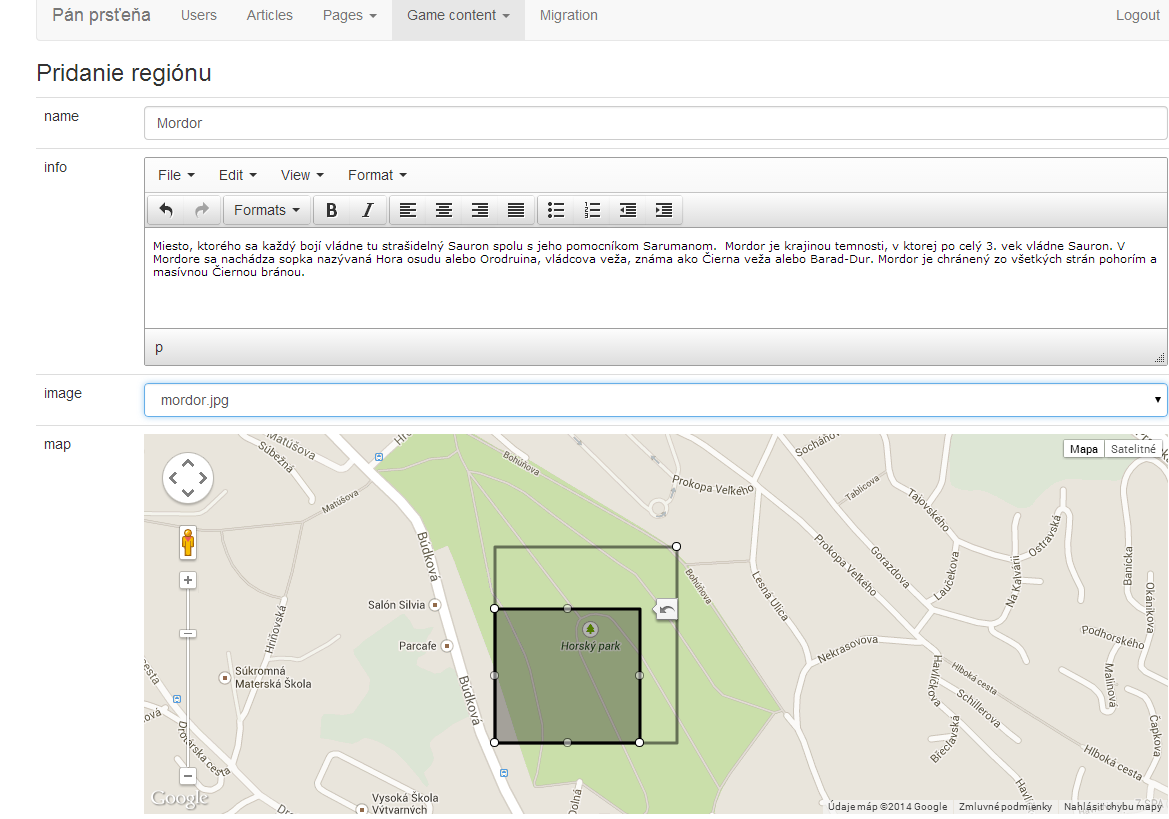
\includegraphics[height=10cm]{mainmatter/imgs/server_pridanieregionu.png}
  \caption{Sekcia na tvorbu a úpravu regiónov}
  \label{fig:server_tvorbaRegionu}
\end{figure}

\section{Členenie hry}
\subsection{Úrovne používateľov}
Z pohľadu možnosti prístupu k serverovej časti aplikácie sa používatelia delia do troch hlavných skupín. 

\subsubsection{Neprihlásený používateľ}
Jedná sa o používateľa s najnižšou právomocou. Má prístup len k verejnym stránkam hry, ktoré by mali obsahovať informácie o hre.

\subsubsection{Hráč}
Je registrovaný a úspešne prihlásený používateľ, ktorý používa mobilnú aplikáciu. Hráč hrá za virtuálnu postavu v hernom svete. Pri pohybe vo svete skutočnom, sa zistí hráčova aktuálna poloha pomocou GPS a je zaslaný dopyt na server s aktuálnou polohou. Zo servera získa vlastnosti herného sveta pre aktuálnu polohu. Hráč môže reagovať na jednotlivé vlastnosti herného sveta - objavovať regióny, hľadať skryté odmeny, plniť rôzne úlohy, či predať ostatným hráčom objekty z herného sveta, ktoré vlastní.

\subsubsection{Administrátor}
Je používateľ webovej aplikácie, ktorý má prístup do administrátorskej sekcie na servery. Tam môže vytvárať, upravovať a mazať jednotlivé vlastnosti herného sveta a hráčov v hernom svete. Tieto vlastnosti môžu byť regióny, úlohy, objekty, atribúty, odmeny ale aj jednotlivé pridelenie a kompletnosť úloh hráčov, či ich atribribúty alebo množstvo predmetov v ich inventároch   vo svete. 

\subsection{Herný svet}
Herný svet je tvorený z regiónov, úloh, objektov, odmien, atribútov a hráčov.

\subsubsection{Regióny}
Herny svet je tvorený regiónmi. Sú to plochy v priestore, v ktorých sa može nachádzať hráč. Každý región má názov, popis a obrázok pre lepšie uvedenie hráča do hry. Hráč pohybom v reálnom svete sa zároveň pohybuje aj v tom hernom. Pomocou mobilnej aplikácie môže vidieť v akých herných regiónoch sa nachádza.

\subsubsection{Úlohy}
Hráč v hernom svete môže plniť úlohy. Môže objaviť dvomi spôsobmi - vstupom do regiónov, na ktoré sú úlohy naviazané, alebo načítaním QR kódov, ktoré im prislúchajú. Po objavení ich môže prijať a následne splniť. Tieto úlohy majú svôj názov, popis a obrázok pre lepšie pochopenie zadania. Úloha môže mať nastavený časový limit, počas ktorého musí byť splnená. Ďalším nastavením úlohy je tzv. autoštart, ktorý automaticky spustí úlohu pre hráča, ktorý vošiel do daného regiónu, na ktorý je naviazaná. Administrátori taktiež majú možnosť naviazať jednotlivé úlohy na seba nastavením požiadavky pre hráčov, ktorí pre spustenie danej úlohy už budú musieť mať splnenú inú - tú, od ktorej je daná úloha zavislá. Úlohy sa podľa spôsobu ich splnenia delia na typy:
\begin{itemize}
	\item Zadanie správnej textovej odpovede
	\item Mať určitú hodnotu atribútu
	\item Nachádzať sa v konkretnom regióne
	\item Vlastniť určité množstvo objektov v inventári
\end{itemize}
Ak má úloha nastavenú odmenu, tak po jej úspešnom splnení ju hráč dostane.


\subsubsection{Objekty, atribúty a odmeny}
\paragraph{Odmeny} sa dajú získať dvomi spôsobmi. Keď hráč úspešne splní úlohu, ktorá má nastavenú odmenu za úspešné splnenie alebo pri nájdení QR kódu, na ktorý je odmena naviazaná. Tak ako pri úlohach, je tiež automaticky vygenerovaný QR kód serverovou aplikáciou pri vytváraní novej odmeny. Odmena môže obsahovať určitý počet objektu a atribútu, ktorý z nej hráč dostane.

\paragraph{Atribúty} sú naviazané na hráčov. Majú svoj názov a obrázok. Každý hráč môže mať určitú hodnotu daného atribútu. Tento herný prvok, by mal byť hlavne využívaný ako prostriedok na porovnávanie medzi hráčmi pri plnení úloh, či nachádzaní odmien. 

\paragraph{Objekty} v hernom svete sa podobajú štruktúrou na atribúty. Tiež majú pomenovanie, obrázok a popisok, v ktorom sa hráči dozvedia k čomu objekt slúži, či jeho príbeh. Objekty, ktoré hráč vlastní uvidí v inventári. Objekty sú taktiež získavané z odmien. Narozdiel od atribútov si hráči medzi sebou môžu objekty odovzdávať. Keď sa teda dvaja hráči dostanú relatívne blízko (na dosah technológie bluetooth), tak môže darca zo svojho inventáru predať druhému spoluhráčovi objekt maximálne o množstve, ktoré darca vlastní.
\begin{figure}[ht!]
  \centering
  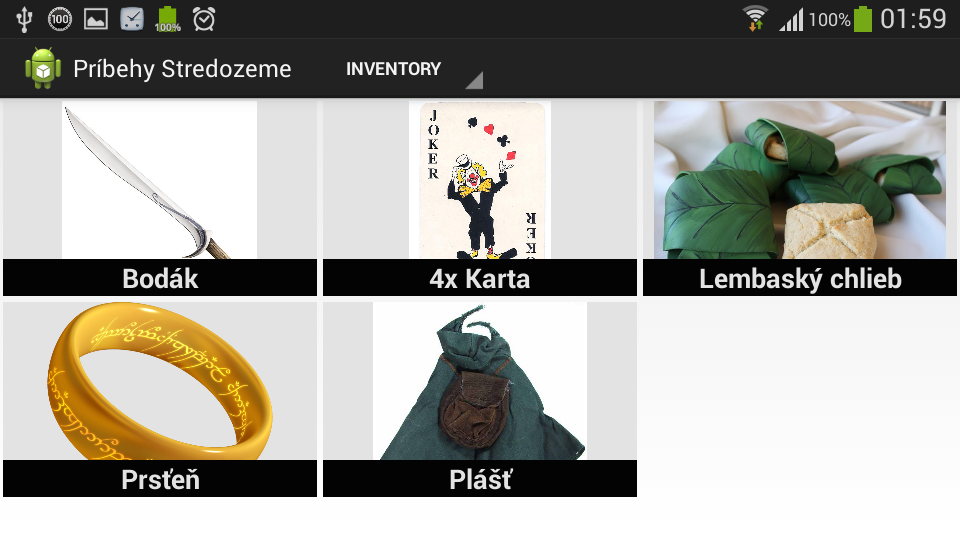
\includegraphics[width=10cm]{mainmatter/imgs/klient_inventory2.png}
  \caption{Inventár hráča}
  \label{fig:klient_inventory}
\end{figure}



\section{Herný príklad}
Hráč sa po uspešnej registrácii prihlási pomocou herného klienta na mobilnom android zariadení do hry. Po úvodnej automatickej synchronizácií herných obrázkov a získaní nastavení hry sa hráčovi zobrazí hlavná obrazovka. Aplikácia, ak nie je nastavené inak, po chvíľke automaticky pošle požiadavku na server a zistí informácie o okolitom hernom prostredí. Hráč zistí, že sa nachádza v bažinách a automaticky  sa mu spustí úloha. V úlohe bude krátky príbeh a zadanie, podľa ktorého má nájsť stratený kameň mudrcov pre vládcu bažín. Po chvíli hľadania hráč nájde QR kód nalepený na kameni. Hráč naskenuje QR kód a dostane informáciu o tom, že sa naozaj jednalo o kameň mudrcov a dostane ho automaticky do inventára. Nájde svoju aktívnu úlohu a stlačí tlačidlo na dokončenie úlohy, keďže splnil zadanie úloha sa označí ako splnená a dostane odmenu. Dostal tri body skúsenosti a jeden meč. Spoluhráč poprosí tohto hráča aby mu predal meč, pretože ho potrebuje na porazenie draka. Prebehne spárovanie zariadení a meč má nového majitela. Hráč pokračuje v plnení úloh, ktoré sú v tomto regióne dostupné. Ďaľšou úlohou je hádanka, ktorú musí uhádnuť a napísať správnu odpoveď. Odpoveď môže zistíť pomocou zozbierania indícií - QR kódov s objektami poschovávaných po okolí. Medzi nimi sa však schovávala nastražená úloha, v ktorej hráč musí újsť pred nahnevanou riečnou príšerou za určitý čas do bezpečia - regiónu, ktorý je obďaleč. Po uspešnom úteku, je hráč odmenený dvomi bodmi fyzickej kóndície. \
Administrátor má tiež prehľad o pohybe hráčov a ich aktuálnych úlohách a inventároch pre lepšiu kontrolu hry. Teda ak vidí, že vznikol problém pri niektorej úlohe, či odmene, môže skrze administrátorskú sekciu webovej aplikácie prideliť objekt, atribút či nastaviť úlohu za hotovú pre konkrétnych hráčov. Môže zmeniť herné prostredie hry počas toho ako jú hráči hrajú. Teda v tomto hernom príklade by si napríklad všimol, že ostatní hráčí nestíhajú dobehnúť do daného regiónu na čas. Tak môže presunúť región bližšie, či nastaviť viac času pre úlohu a dať za ňu nižšiu odmenu.

\paragraph{}
Z hernej ukážky môžeme povedať, že vysledné hry budú môcť čerpať časť čŕt z larpov, kde sa hráči vžíjú do svojich postáv a prechádzajú určitým príbehom \cite{larp-cojeto}. Tiež geocachingu, kde hráči hľadajú kešky(správy či iné malé objekty), ktoré pre nich zanechali ostatní na určitej GPS pozícii \cite{geocaching}. Veľkú podobnosť možme nájst aj so šifrovacími hrami. 

\section{Minimálne požiadavky}
\subsection{Klient}
\begin{itemize}
\item Aby sa hráči mohli pripojiť na herný server a mohli hrať hry vytvorené pomocou tohto frameworku potrebujú mobilné zariadenie s operačným systémom Android o minimálnej verzii 2.3 s označením Gingerbread. 
\item Na zariadení je potrebné mať aspoň 8,5MB volného miesta na inštaláciu samostatnej aplikácie bez herného obsahu. Čiže celkové požiadavky na pamäť sa líšia podla jednotlivého serveru, na ktorom je klient pripojený. 
\item Potrebné je tiež pripojenie k internetu, vďaka ktorému dochádza ku komunikácii s herným serverom a teda získavaní informácií o hernom svete a interagovaní s ním. 
\item Tiež velmi podstatnou súčasťou požiadaviek je aby dané mobilné zariadenie bolo vybavené fotoaparátom, aby bolo schopné rozoznať QR kódy. 
\item Pre plnohodnotné využitie hry, je tiež potrebný GPS sensor z dôvodu udávania presnej polohy hráča a tak releventných informácii o prostredí zavislých na polohe. 
\item Bluetooth technológia je potrebná pre zdielanie objektov medzi hráčmi. 
\end{itemize}

\subsection{Server}
Aplikácia pre svoj správny beh na strane servera potrebuje:
\begin{itemize}
\item PHP verzie 5.1.6 alebo novší \cite{codeigniter-requirements}
\item MySQL databázu 4.1+ alebo novšiu \cite{codeigniter-requirements}
\item GD2 knižnicu pre tvorbu QR kódov \cite{qrgenerator-info}
\item minimálne 3,5MB na disku (bez herného obsahu)
\end{itemize}

\section{Spôsoby riešenia problémov}
\subsection{Tvorba herného sveta}
Jedným z hlavných problémov bolo navrhnúť prostredie pre tvorcov hry, ktoré nebude vyžadovať programátorské schopnosti. Zároveň by však malo ponúknuť tvorcom hry dostatočnú volnosť a možnosť jednoduchej spolupráci pri tvorbe herného sveta. Preto najlepším riešením bola webová aplikácia, ktorá je súčasťou frameworku. Administrátori cez jednotlivé nástroje na tvorbu a úpravu herného obsahu teda môžu jednoducho vytvoriť hru. 

\subsection{Univerzálnosť klienta}
Pri obsahovo rôznych hrách vytvorených pomocou frameworku na strane servera vznikol, problém univerzálnosti klienta. Klient musí byť bez externých zásahov kompatibilný so všetkými hrami vytvorenými webovou aplikáciou frameworku. Preto si klient po úspešnom pripojení a prihlásení stiahne nastavenia hry a chýbajúce obrázky z herného serveru. Zároveň cieľom návrhu výzoru klienta bola, čo najmenšia konfliktnosť s možným obsahom hry.

\subsection{Komunikacia klient-server}
Na serveri v databázových moodeloch sa už ukrýva virtuálny svet hry, avšak klient nemá žiadne informácie o hre na danom serveri. Preto bolo nevyhnutné navrhnúť spôsob komunikácie medzi týmito dvomi stranami. Ako najlepšie možné riešenie bola zvolená komunikácia z klientovej strany pomocou požiadaviek POST a GET, pomocou ktorých sa volá herné API na strane servera. Server na tieto požiadavky posiela textové odpovede vo formáte JSON. Javascriptová objektová notácia má mnohé výhody, pre ktoré je použitá na komunikáciu. Napríklad oproti XML formátu má JSON velkosť často menšiu velkosť a rýchlosť spracovania je vyššia. \cite{jsonVsXml} Ďaľšou podstatnou vlastnosťou je nezávislosť formátu na počítačovej platforme a množstvo knižníc, ktoré ulahčujú prácu pri spracovaní dát v tomto formáte.

\subsection{Vytvorenie redakčného systému}
Jedným z ďaľších problémov, bola potreba informovať potenciálnych hráčov o hre. Ponúknuť im príbehy z prostredia, v ktorom sa hra odohráva a aj návod ako začať hru hrať, teiž kde a kedy sa hra odohráva. Ďaľším podstatným dôvodom bolo informovať hráčov o novinkách a upozorneniach v hre. Preto bolo potrebné riešenie, kde používateľ (administrátor) by bez potreby inštalácie redakčných systémov môže vytvárať a upravovať stránky o hre. Toto sa podarilo pomocou jednoduchého vstavaného WYSIWYG HTML editora  tj. editora, ktorý sa snaží ponúknuť tvorcovi verný obraz výzoru výslednej stránky počas jej tvorby.

\subsection{Spušťanie pomocou QR kódov}

Definícia regiónov pomocou GPS súradníc, ponúka veľkú výhodu - možnosť hrať hru vonku v teréne. Avšak pri potrebe zadania úloh v miestach so slabým GPS signálom napríklad v budovách, či schovávania herných odmien vzniká problém. Tento problém riešia kódy, ktoré sú unikátne pre každú odmenu a úlohu. Teda webová aplikácia v administračnej sekcii automaticky vygeneruje kód, ktorý administrátorovi ponúkne ako QR kód pre načítanie klientom. Výhodou tohto riešenia je prínos nových možností ako vystavať herné zážitky - možnosť schovania odmien, či ponúknutia úloh. Nevýhodou je aby mobilné zariadenie malo fotoaparát, pomocou ktorého sú QR kódy skenované. QR kódy ponúkajú možnosť zakódovania informácie tak, aby ich prečítanie bolo možné aj pri poškodení časti QR kódu až do približne 30\% obrázku \cite{qr-error}. Túto vlastnosť možno využiť na prisposobenie výsledných QR kódov prekrytím ich časti logom s názvom hry.

\begin{figure}[h]
  \centering
  
\includegraphics[height=10cm]{mainmatter/imgs/qrcode.png}
  \caption{Čitatelný QR kód s logom hry}
  \label{fig:qrcode}
\end{figure}


\subsection{Komunikácia medzi hráčmi}
Pre splnenie úlohy môže hráč potrebovať objekt, ktorý získal druhý hráč. Takto môžu vznikať tímy, ktoré si pomáhajú v plnení úloh. Tu vzniká problém aký spôsob komunikácie medzi klientami zvoliť. Naskytá sa možnosť priameho dopytu na herné API na serveri od darcu pre darovanie objektu. Tu však vzniká problém, že hráči by mohli byť od seba veľmi ďaleko, čo kazí herný zážitok. Tento problém môžeme ošetriť kontrolou polohy oboch hráčov, toto riešenie by však nefungovalo v priestoroch kde je GPS signal slabší. Preto do úvahy pripadli technológie NFC a Bluetooth. Problém pri NFC je, že sa jedná o relatívne mladú technológiu a preto by sa minimálne nároky na klienta zdvihli, potrebou vlastniť mobilné zariadenie, ktoré by podporovalo túto technológiu, ktorú mnohé staršie zariadenia nemajú. Preto bol zvolený Bluetooth na komunikáciu medzi zariadeniami, pretože sa jedná o dlhšie zaužívanú technológiu pri mobilných zariadeniach.



